Your task is to build the interpreter for Assembly SVM. This means that the template will generate a data structure representing the program, as defined in the module \texttt{SVMAST}, and you will have to build a software that executes that code, according to the instruction set defined above. Your program should be able to accept as input the source file written in Assembly SVM and the size (number of addresses) of the memory of the SVM you want to run the program on. The interpreter should raise an exception (which must be captured appropriately) in case of incompatible arguments, as described in the instruction behaviour. The output of the program should be a \textit{dump} of the SVM, which contains a visualization of the memory, the registers, and the program counter. Organize the memory display as a table with the memory locations content with 10 items per row. An example of a memory dump is shown in Figure \ref{fig:dump}.

\begin{figure}
	\centering
	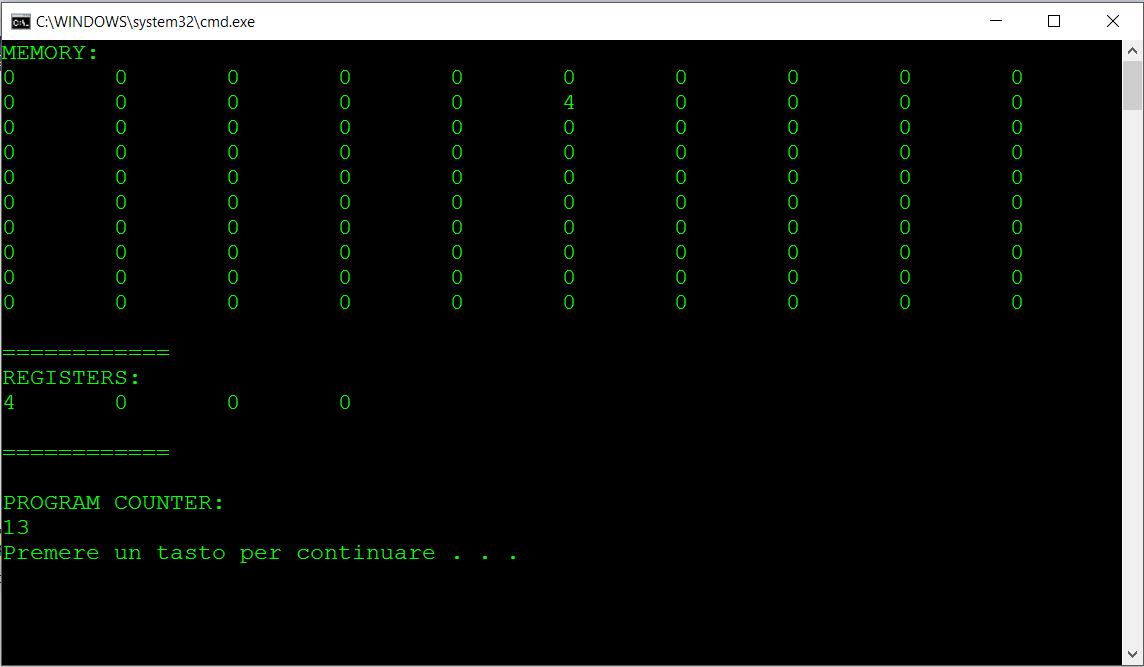
\includegraphics[width = \textwidth]{Figures/dump}
	\caption{Memory dump}
	\label{fig:dump}
\end{figure}

\noindent
Your implementation must observe the following rules:

\begin{itemize}
	\item You are not allowed to use any imperative constructs, other than statements that print on the standard output (such as \texttt{printfn}) and exceptions (\texttt{try-with} and \texttt{exception} definitions). This means no mutable values (\texttt{let mutable}), no variable assignments, such as \texttt{let mutable x = 0; x <- x + 1}, no \texttt{classes} (although immutable records are allowed), no \texttt{for} or \texttt{while} loops (you can use \textit{list comprehension} if you understand how they work, but this is out of the scope of the course), no arrays (only lists). You are allowed to use methods and properties in conjunction with  immutable records if they behave in an immutable way (so if they respect the constraints above).
	\item Your implementation should show that you know as much as possible the constructs of functional programming, so use as much as possible (of course where it makes senese) higher order functions, tuples, discriminated unions, immutable records, etc.
	\item Your solution must be tested with the examples included in the template but you are allowed to add your own programs written in Assembly SVM and present them.
	\item You are not allowed to change any part of the language definition, that is, the grammar, the syntactical representation generated by the Parser, and the instruction set.
\end{itemize}

\subsection{Evaluation}
Below you find how the evaluation matrix

\begin{longtable}{|c|c|p{8cm}|}
	\hline
	\textbf{Feature} & Maximum score & Details \\
	\hline
	SVM representation & 2 & The SVM is structured using a record with appropriate methods, properties, or functions implementing the functionalities (2 points). The SVM is implemented but without an explicit data type (1 point) or functions are not well structured according to the functional paradigm. 0 otherwise \\
	\hline
	Operators & 4 & Boolean, arithmetic, and comparison operators are implemented correctly (4 points). Operators are implemented but the exceptions are not handled properly or the argument by reference does not work (2 points). 0 otherwise. \\
	\hline
	Jump & 4 & Jump operators and labels are correctly implemented (4 points). Some jump operators are missing or not fully working (2 points). 0 otherwise. \\
	\hline  
\end{longtable}